%%%%%%%%%%%%%%%%%%%%%%%%%%%%%%%%%%%%%%%%%
% Masters/Doctoral Thesis
% LaTeX Template
% Version 1.43 (17/5/14)
%
% This template has been downloaded from:
% http://www.LaTeXTemplates.com
%
% Original authors:
% Steven Gunn
% http://users.ecs.soton.ac.uk/srg/softwaretools/document/templates/
% and
% Sunil Patel
% http://www.sunilpatel.co.uk/thesis-template/
%
% License:
% CC BY-NC-SA 3.0 (http://creativecommons.org/licenses/by-nc-sa/3.0/)
%
% Note:
% Make sure to edit document variables in the Thesis.cls file
%
%%%%%%%%%%%%%%%%%%%%%%%%%%%%%%%%%%%%%%%%%

%----------------------------------------------------------------------------------------
%	PACKAGES AND OTHER DOCUMENT CONFIGURATIONS
%----------------------------------------------------------------------------------------

\documentclass[11pt, oneside]{Thesis} % The default font size and one-sided printing (no margin offsets)

\graphicspath{{Pictures/}} % Specifies the directory where pictures are stored

\usepackage[square, numbers, comma, sort&compress]{natbib} % Use the natbib reference package - read up on this to edit the reference style; if you want text (e.g. Smith et al., 2012) for the in-text references (instead of numbers), remove 'numbers'
\hypersetup{urlcolor=blue, colorlinks=true} % Colors hyperlinks in blue - change to black if annoying
\title{\ttitle} % Defines the thesis title - don't touch this

\begin{document}

\frontmatter % Use roman page numbering style (i, ii, iii, iv...) for the pre-content pages

\setstretch{1.3} % Line spacing of 1.3

% Define the page headers using the FancyHdr package and set up for one-sided printing
\fancyhead{} % Clears all page headers and footers
\rhead{\thepage} % Sets the right side header to show the page number
\lhead{} % Clears the left side page header

\pagestyle{fancy} % Finally, use the "fancy" page style to implement the FancyHdr headers

\newcommand{\HRule}{\rule{\linewidth}{0.5mm}} % New command to make the lines in the title page

% PDF meta-data
\hypersetup{pdftitle={\ttitle}}
\hypersetup{pdfsubject=\subjectname}
\hypersetup{pdfauthor=\authornames}
\hypersetup{pdfkeywords=\keywordnames}

%----------------------------------------------------------------------------------------
%	TITLE PAGE
%----------------------------------------------------------------------------------------

\begin{titlepage}
\begin{center}

\textsc{\LARGE \univname}\\[1.5cm] % University name
\textsc{\Large Doctoral Thesis}\\[0.5cm] % Thesis type

\HRule \\[0.4cm] % Horizontal line
{\huge \bfseries \ttitle}\\[0.4cm] % Thesis title
\HRule \\[1.5cm] % Horizontal line

\begin{minipage}{0.4\textwidth}
\begin{flushleft} \large
\emph{Author:}\\
\href{http://www.johnsmith.com}{\authornames} % Author name - remove the \href bracket to remove the link
\end{flushleft}
\end{minipage}
\begin{minipage}{0.4\textwidth}
\begin{flushright} \large
\emph{Supervisor:} \\
\href{http://www.jamessmith.com}{\supname} % Supervisor name - remove the \href bracket to remove the link
\end{flushright}
\end{minipage}\\[3cm]

\large \textit{A thesis submitted in fulfilment of the requirements\\ for the degree of \degreename}\\[0.3cm] % University requirement text
\textit{in the}\\[0.4cm]
\groupname\\\deptname\\[2cm] % Research group name and department name

{\large \today}\\[4cm] % Date
%\includegraphics{Logo} % University/department logo - uncomment to place it

\vfill
\end{center}

\end{titlepage}

%----------------------------------------------------------------------------------------
%	DECLARATION PAGE
%	Your institution may give you a different text to place here
%----------------------------------------------------------------------------------------

\Declaration{

\addtocontents{toc}{\vspace{1em}} % Add a gap in the Contents, for aesthetics

I, \authornames, declare that this thesis titled, '\ttitle' and the work presented in it are my own. I confirm that:

\begin{itemize}
\item[\tiny{$\blacksquare$}] This work was done wholly or mainly while in candidature for a research degree at this University.
\item[\tiny{$\blacksquare$}] Where any part of this thesis has previously been submitted for a degree or any other qualification at this University or any other institution, this has been clearly stated.
\item[\tiny{$\blacksquare$}] Where I have consulted the published work of others, this is always clearly attributed.
\item[\tiny{$\blacksquare$}] Where I have quoted from the work of others, the source is always given. With the exception of such quotations, this thesis is entirely my own work.
\item[\tiny{$\blacksquare$}] I have acknowledged all main sources of help.
\item[\tiny{$\blacksquare$}] Where the thesis is based on work done by myself jointly with others, I have made clear exactly what was done by others and what I have contributed myself.\\
\end{itemize}

Signed:\\
\rule[1em]{25em}{0.5pt} % This prints a line for the signature

Date:\\
\rule[1em]{25em}{0.5pt} % This prints a line to write the date
}

\clearpage % Start a new page

%----------------------------------------------------------------------------------------
%	QUOTATION PAGE
%----------------------------------------------------------------------------------------

\pagestyle{empty} % No headers or footers for the following pages

\null\vfill % Add some space to move the quote down the page a bit

\textit{``Thanks to my solid academic training, today I can write hundreds of words on virtually any topic without possessing a shred of information, which is how I got a good job in journalism."}

\begin{flushright}
Dave Barry
\end{flushright}

\vfill\vfill\vfill\vfill\vfill\vfill\null % Add some space at the bottom to position the quote just right

\clearpage % Start a new page

%----------------------------------------------------------------------------------------
%	ABSTRACT PAGE
%----------------------------------------------------------------------------------------

\addtotoc{Abstract} % Add the "Abstract" page entry to the Contents

\abstract{\addtocontents{toc}{\vspace{1em}} % Add a gap in the Contents, for aesthetics

The Thesis Abstract is written here (and usually kept to just this page). The page is kept centered vertically so can expand into the blank space above the title too\ldots
}

\clearpage % Start a new page

%----------------------------------------------------------------------------------------
%	ACKNOWLEDGEMENTS
%----------------------------------------------------------------------------------------

\setstretch{1.3} % Reset the line-spacing to 1.3 for body text (if it has changed)

\acknowledgements{\addtocontents{toc}{\vspace{1em}} % Add a gap in the Contents, for aesthetics

The acknowledgements and the people to thank go here, don't forget to include your project advisor\ldots
}
\clearpage % Start a new page

%----------------------------------------------------------------------------------------
%	LIST OF CONTENTS/FIGURES/TABLES PAGES
%----------------------------------------------------------------------------------------

\pagestyle{fancy} % The page style headers have been "empty" all this time, now use the "fancy" headers as defined before to bring them back

\lhead{\emph{Contents}} % Set the left side page header to "Contents"
\tableofcontents % Write out the Table of Contents

\lhead{\emph{List of Figures}} % Set the left side page header to "List of Figures"
\listoffigures % Write out the List of Figures

\lhead{\emph{List of Tables}} % Set the left side page header to "List of Tables"
\listoftables % Write out the List of Tables

%----------------------------------------------------------------------------------------
%	ABBREVIATIONS
%----------------------------------------------------------------------------------------

\clearpage % Start a new page

\setstretch{1.5} % Set the line spacing to 1.5, this makes the following tables easier to read

\lhead{\emph{Abbreviations}} % Set the left side page header to "Abbreviations"
\listofsymbols{ll} % Include a list of Abbreviations (a table of two columns)
{
\textbf{LAH} & \textbf{L}ist \textbf{A}bbreviations \textbf{H}ere \\
%\textbf{Acronym} & \textbf{W}hat (it) \textbf{S}tands \textbf{F}or \\
}

%----------------------------------------------------------------------------------------
%	PHYSICAL CONSTANTS/OTHER DEFINITIONS
%----------------------------------------------------------------------------------------

\clearpage % Start a new page

\lhead{\emph{Physical Constants}} % Set the left side page header to "Physical Constants"

\listofconstants{lrcl} % Include a list of Physical Constants (a four column table)
{
Speed of Light & $c$ & $=$ & $2.997\ 924\ 58\times10^{8}\ \mbox{ms}^{-\mbox{s}}$ (exact)\\
% Constant Name & Symbol & = & Constant Value (with units) \\
}

%----------------------------------------------------------------------------------------
%	SYMBOLS
%----------------------------------------------------------------------------------------

\clearpage % Start a new page

\lhead{\emph{Symbols}} % Set the left side page header to "Symbols"

\listofnomenclature{lll} % Include a list of Symbols (a three column table)
{
$a$ & distance & m \\
$P$ & power & W (Js$^{-1}$) \\
% Symbol & Name & Unit \\

& & \\ % Gap to separate the Roman symbols from the Greek

$\omega$ & angular frequency & rads$^{-1}$ \\
% Symbol & Name & Unit \\
}

%----------------------------------------------------------------------------------------
%	DEDICATION
%----------------------------------------------------------------------------------------

\setstretch{1.3} % Return the line spacing back to 1.3

\pagestyle{empty} % Page style needs to be empty for this page

\dedicatory{For/Dedicated to/To my\ldots} % Dedication text

\addtocontents{toc}{\vspace{2em}} % Add a gap in the Contents, for aesthetics

%----------------------------------------------------------------------------------------
%	THESIS CONTENT - CHAPTERS
%----------------------------------------------------------------------------------------

\mainmatter % Begin numeric (1,2,3...) page numbering

\pagestyle{fancy} % Return the page headers back to the "fancy" style

% Include the chapters of the thesis as separate files from the Chapters folder
% Uncomment the lines as you write the chapters

% Chapter 1
\chapter{Fundamental Mathematics} % Main chapter title

\label{Chapter1} % For referencing the chapter elsewhere, use \ref{Chapter1}

\lhead{Chapter 1. \emph{Fundamental Mathematics}} % This is for the header on each page - perhaps a shortened title

%----------------------------------------------------------------------------------------
\section{Linear algebra}
\begin{compactitem}

\item {Diagonal Matrix Properties}
In linear algebra, a diagonal matrix is a matrix (usually a square matrix) in which
the entries outside the main diagonal are all zero. The diagonal entries themselves
may or may not be zero. Thus, the matrix $D = (d_{i,j})$ with n columns and n rows is diagonal
if:
$d_{i,j}=0,\, if \,\, i \neq j \,\, \forall i,j \in \{1,2,3,...n\} $
\\For example, the following matrix is diagonal:\\
$\begin{pmatrix}
       1	&0 	&0	\\[0.3em]
       0 	&4 	&0 	\\[0.3em]
       0 	& 0 	&-2	\\[0.3em]
\end{pmatrix}
$ \cite{wiki-Diagonal_matrix}
\\
\\The general form :$D=diag(\lambda_{ii}) =$
\begin{equation}
\label{eq:diagm}
\begin{pmatrix}
       \lambda_{00}& 0 				& ..	&	0 	\\[0.3em]
       0 			& \lambda_{11} & ..		&	0 	\\[0.3em]
       .			& .				& ..	&	.	\\[0.3em]
       0 			& 0 			& ..	&	\lambda_{nn}\\[0.3em]
     \end{pmatrix}
\end{equation}

\begin{equation}
\label{eq:pdpD}
D^{-1}=diag(\lambda_{ii}^{-1})=
\begin{pmatrix}
       1/\lambda_{00}& 0 				& ..	&	0 	\\[0.3em]
       0 			& 1/\lambda_{11} & ..		&	0 	\\[0.3em]
       .			& .				& ..	&	.	\\[0.3em]
       0 			& 0 			& ..	&	1/\lambda_{nn}\\[0.3em]
\end{pmatrix}
, \forall \Lambda_{ii} \neq 0,
\end{equation}\\

The determinant of a Diagonal matrix is the product of all the diagonal elements.
\begin{equation}
\label{eq:detD}
det(D) = \prod_{i}^{} \lambda_{ii}
\end{equation}

\begin{equation}
\label{eq:det-pdpD}
\\
det(D^{-1})=
\prod_{i}^{} \frac{1}{\lambda_{ii} }\\
=\prod_{i}^{} \lambda_{ii}^{-1} \\
\end{equation}\\

%----------------------------------------------------------------------------------------
\item {Eigen Values and Eigen Vectors}
\\If A is a n*n square matrix. Eigen value $\lambda$ and \textbf{eigen} vector $\hat{x}$: \cite{AntonELA10th}
\begin{equation}
\label{eq:eval}
A\hat{x}=\lambda \hat{x}
\end{equation}
The sign of $\lambda$ and $\hat{x}$ are not unique. And $\lambda$ and $\hat{x}$ are scalable.
\\$ (A-\lambda I)X=0$
Set the determinant to zero to obtain the polynomial equation to solve the eigen values.
$det(A-\lambda I)=0$

\item singular value decomposition
\\U and V are orthogonal matrix, $U^{-1}=U^{\top}, V^{-1}=V^{\top}$\\
r=rank A
\begin{flalign}
\underbrace{\mathbf{A}}_{M \times N} = \underbrace{\mathbf{U}}_{M \times M} \times
\underbrace{\mathbf{\Sigma}}_{M\times N} \times
\underbrace{\mathbf{V}^{\text{T}}}_{N \times N} = &
\end{flalign}

\hspace*{-3cm}\vbox{
\begin{flalign}
\begin{tikzpicture}[
baseline,
mymat/.style={
  matrix of math nodes,
  ampersand replacement=\&,
  left delimiter=(,
  right delimiter=),
  nodes in empty cells,
  nodes={outer sep=-\pgflinewidth,text depth=0.5ex,text height=2ex,text width=1.2em}
}
]
\begin{scope}[every right delimiter/.style={xshift=-3ex}]
\matrix[mymat] (matu)
{
 \& \& \& \& \& \\
\& \& \& \& \& \\
\& \& \& \& \& \\
\& \& \& \& \& \\
\& \& \& \& \& \\
\& \& \& \& \& \\
};
\node
  at ([shift={(3pt,-7pt)}]matu-3-2.west)
  {$\cdots$};
\node
  at ([shift={(3pt,-7pt)}]matu-3-5.west)
  {$\cdots$};
\foreach \Columna/\Valor in {1/1,3/r,4/{r+1},6/m}
{
\draw
  (matu-1-\Columna.north west)
    rectangle
  ([xshift=4pt]matu-6-\Columna.south west);
\node[above]
  at ([xshift=2pt]matu-1-\Columna.north west)
  {$u_{\Valor}$};
}
\draw[decorate,decoration={brace,mirror,raise=3pt}]
  (matu-6-1.south west) --
   node[below=4pt] {$\Mcol(A)$}
  ([xshift=4pt]matu-6-3.south west);
\draw[decorate,decoration={brace,mirror,raise=3pt}]
  (matu-6-4.south west) --
   node[below=4pt] {$\Mnull(A)$}
  ([xshift=4pt]matu-6-6.south west);
\end{scope}
\matrix[mymat,right=10pt of matu] (matsigma)
{
\sigma_{1} \& \& \& \& \& \\
\& \ddots \& \& \& \& \\
\& \& \sigma_{r} \& \& \& \\
\& \& \& 0 \& \& \\
\& \& \& \& \ddots \& \\
\& \& \& \& \& 0 \\
};
%\begin{scope}[every right delimiter/.style={xshift=-3ex}]
\matrix[mymat,right=25pt of matsigma] (matv)
{
 \& \& \& \& \& \\
\& \& \& \& \& \\
\& \& \& \& \& \\
\& \& \& \& \& \\
\& \& \& \& \& \\
\& \& \& \& \& \\
};
\foreach \Fila/\Valor in {1/1,3/r,4/{r+1},6/n}
{
\draw
  ([yshift=-6pt]matv-\Fila-1.north west)
    rectangle
  ([yshift=-10pt]matv-\Fila-6.north east);
\node[right=12pt]
  at ([yshift=-8pt]matv-\Fila-6.north east)
  {$v^{T}_{\Valor}$};
}
\draw[decorate,decoration={brace,raise=37pt}]
  ([yshift=-6pt]matv-1-6.north east) --
   node[right=38pt] {$\Mrow(A)$}
  ([yshift=-10pt]matv-3-6.north east);
\draw[decorate,decoration={brace,raise=37pt}]
  ([yshift=-6pt]matv-4-6.north east) --
   node[right=38pt] {$\Mnull(A)$}
  ([yshift=-10pt]matv-6-6.north east);
\end{tikzpicture}
\end{flalign}}

%----------------------------------------------------------------------------------------
\item {Symmetric Matrix:}\\
A symmetric matrix is a square matrix that is equal to its transpose.
Formally, matrix A is symmetric if $A = A^{\top}$.
So if the entries are written as $A = (a_{ij}), \,then\,\, a_{ij} = a_{ji}$.
\\
A real sqaure symmetric matrix can be Eigen Value Decomposition : $A=PDP^{\top}$.
D is a diagonal matrix whose elements are eigen values of A.
P is composed of orthogonal eigen vectors, so $P^{-1}=P^{\top}$.\\
\begin{equation}
\label{eq:pdpI}
I=P* P^{-1} = P* P^{\top}
\end{equation}

\item positive definite matrix : $x^{\top} A x \geq 0 ,\forall\, x \, \in \, \mathbb{R}^{N}$
\\
Every positive definite matrix has positive eigenvalues.


\end{compactitem}
%----------------------------------------------------------------------------------------

\section{Covariance and Whitening}
\begin{compactitem}

\item {standard deviation and variance}
\begin{equation}
\label{eq:std}
\sigma = \sqrt {\sum \frac{(x-\bar{x})^2}{N}}
\end{equation}
\begin{equation}
\label{eq:variance}
VAR(X)=\sigma^{2} = {\sum \frac{(x-\bar{x})^2}{N}}
\end{equation}

\item covariance: X and Y are two vectors, random variables. The covariance is a value.
\begin{equation}
\label{eq:covar}
Cov(X,Y)=\sigma(X,Y)=E[(X - E[X])(Y-E[Y])] \\
Cov(X,Y)=\frac{\sum(X_i-\bar{X})(Y_i-\bar{Y})}{N}=
\frac{\sum(x_i)(y_i)}{N}
\end{equation}

Deviation score $x_i, y_i$:
\begin{equation}
\label{eq:covar1}
x_{i}=(X_i-\bar{X}),\;
y_{i}=(Y_i-\bar{Y})
\end{equation}
Variance of X, $VAR(X)=Cov(X,X)=\sigma^{2}$, \ is a degenerated form of covariance.\\

\item {covariance matrix:}
is a measure of the extent to which corresponding elements from two sets
of ordered data move in the same direction. We use the following formula to compute covariance.
\cite{wiki-covariance}\cite{STAT-covariance}\\
\\Let $X_i$ be the \textbf{column} vector in a Matrix \textbf{X}=
$\begin{pmatrix} X_1 & X_2 &... & X_c \end{pmatrix}$\\
The covariance matrix of \textbf{X} is:\\
$M_{cxc} = \Sigma{(\textbf{X})}=$
\[
\begin{pmatrix}
       COV(X_1,X_1) 	& COV(X_1,X_2) 	& ...	& COV(X_1,X_c)	\\[0.3em]
       COV(X_2,X_1) 	& COV(X_2,X_2) 	& ...	& COV(X_2,X_c)	\\[0.3em]
       ...		& ...			& ...	&	...		\\[0.3em]
       COV(X_c,X_1) 	& COV(X_c,X_2) 	& ...	& COV(X_c,X_c)	\\[0.3em]
\end{pmatrix}
=\]
\begin{equation}
\label{eq:covarm1}
\begin{pmatrix}
       \sum x_{1i}^{2}/N 	& \sum x_{1i} x_{2i}/N 	& ...	& \sum x_{1i} x_{ci}/N	\\[0.3em]
       \sum x_{2i} x_{1i}/N 	& \sum x_{2i} x_{2i}/N 	& ...	& \sum x_{2i} x_{ci}/N	\\[0.3em]
       ...		& ...			& ...	&	...		\\[0.3em]
       \sum x_{ci} x_{1i}/N 	& \sum x_{ci} x_{2i}/N 	& ...	& \sum x_{ci}^{2}/N	\\[0.3em]
\end{pmatrix}
=(1/N)
\begin{pmatrix}
       \sum x_{1i}^{2} 	& \sum x_{1i} x_{2i} 	& ...	& \sum x_{1i} x_{ci}	\\[0.3em]
       \sum x_{2i} x_{1i} 	& \sum x_{2i} x_{2i} 	& ...	& \sum x_{2i} x_{ci}	\\[0.3em]
       ...		& ...			& ...	&	...		\\[0.3em]
       \sum x_{ci} x_{1i} 	& \sum x_{ci} x_{2i} 	& ...	& \sum x_{ci}^{2}	\\[0.3em]
\end{pmatrix}
\end{equation}
where\\
N is the dim of the column vector $X_i$.\\
$x_i$ is a deviation score from the ith data set.\\
$\sum x_i^2 / N$ is the variance of elements from the ith data set.\\
$\sum x_i x_j / N$ is the covariance for elements from the ith and jth data sets.\\

\item Properties of Covariance matrix :
\textbf{square, symmetric and positive semidefinite}: \\
Eigen value decomposition for a \textbf{square, symmetric} matrix:
\begin{equation}
\label{eq:covd}
\Sigma(\textbf{X}) = U\Lambda U^T
\end{equation}


When A is positive semi-definite, $x^T A x >= 0$ and all eigen values are positive.  $\Sigma(\textbf{X})$ has all positive eigen values.

Diagonal matrix $\Lambda$ has all positive eigen values in its diagonal elements. $\Lambda ^ {1/2}$ doest exist and $\Lambda ^ {-1/2}$ doest exist, too.\\

\textbf{linearity of expectation matrix}: Let \textbf{X} be a random vector with covariance matrix
$\Sigma(\textbf{X})$, and let A be a matrix that can act on \textbf{X}. The covariance matrix of the vector A\textbf{X} is:
\begin{equation}
\label{eq:covlinear}
\Sigma(A\textbf{X}) = A\Sigma(\textbf{X})A^{T}
\end{equation}

\item whiten: Refer to \eqref{eq:covd},  A \textbf{whitening} matrix W is defined as
\begin{equation}
\label{eq:whitem}
W=U\Lambda^{-1/2} U^{T}
\end{equation}
This W is not unique, because $\Lambda$ and $U^T$ are not unique.
When the diagonal elements, eigen value, of the diagonal matrix, $\Lambda$, are changed in the order.
$U$ is also changed .

Let X and Y are \textbf{row-major} matrix, i.e, signals are in row vectors.
\begin{equation}
\label{eq:whitened}
Y_{nm} = W_{nn}*\textbf{X}_{nm}= (U\Lambda^{-1/2} U^{T}) \textbf{X}_{nm}
\end{equation}
Sometimes, column-major is used in fortran and some math tools,
\begin{equation}
\label{eq:whitened-col}
Y' = (W_{nn}*\textbf{X}_{nm})' = \textbf{X}'*W'= \textbf{X}*(U\Lambda^{-1/2} U^{T})'=\textbf{X}*(U^{T}\Lambda^{-1/2} U)
\end{equation}
be a \textbf{whitened matrix} of \textbf{X}.\\
The covariance matrix of Y which is a whitened matrix of X.
\[
\Sigma (Y)=\Sigma (U\Lambda^{-1/2} U^{T}) \textbf{X}
\]
Refer to the equation \eqref{eq:covlinear}
\[
A=(U\Lambda^{-1/2} U^{T})
\]
so
\[
\Sigma (Y)=\Sigma (U\Lambda^{-1/2} U^{T}) \textbf{X}=
(U\Lambda^{-1/2} U^{T})(\Sigma (\textbf{X})) (U\Lambda^{-1/2} U^{T})^{T}
\]
Refer to the equation \eqref{eq:covd}\\
$=(U\Lambda^{-1/2} U^{T}) (U \Lambda U^{T}) (U\Lambda^{-1/2} U^{T}) ^T$\\
$=U\Lambda^{-1/2} (U^{T}  U) \Lambda U^{T} (U\Lambda^{-1/2} U^{T}) ^T$\\
Refer to the equation \eqref{eq:pdpI}\\
$=U\Lambda^{-1/2} (I) \Lambda U^{T} ({U^{T}}^T{\Lambda^{-1/2}}^T U^T)$\\
$=U\Lambda^{-1/2} \Lambda U^{T} (U{\Lambda^{-1/2}}^T) U^T$\\
$=U\Lambda^{-1/2} \Lambda (U^{T} U) {\Lambda^{-1/2}}^T U^T$\\
$=U\Lambda^{-1/2} \Lambda (I) {\Lambda^{-1/2}}^T U^T$\\
$=U\Lambda^{-1/2} \Lambda \Lambda^{-1/2} U^T$\\
$=U\Lambda^{(-1/2) + (1) + (-1/2)} U^T$\\
$=U I U^T = U U^T = I $\\
So \textbf{Y is whitened}, because its covariance matrix is an Identity matrix.
All row vectors in Y has no correlation!

\item \textbf{Simplification} for a \textbf{normalized} vector $\hat{X_i}$:\\
Let \textbf{X}=$\begin{pmatrix} X_1 & X_2 & ... & X_c \end{pmatrix}, X_1,X_2,X_c$ are column vectors which have been normalized.
(zero mean )\\

Refer to the equation \eqref{eq:covar1}, Deviation score $x_k, y_k$:\\
$x_{k}=(X_{ik}-\bar{X_i})=(X_{ik} - 0)= X_{ik}$ \\
$y_{k}=(Y_{ik}-\bar{Y_i})=(Y_{ik} - 0) = Y_{ik}$


Refer to the equation \eqref{eq:covarm1}, covariance matrix $\Sigma(\textbf{X})$=
\[
(1/N)
\begin{pmatrix}
       \sum x_{1k}^{2} 	& \sum x_{1k} x_{2k} 	& ...	& \sum x_{1k} x_{ck}	\\[0.3em]
       \sum x_{2k} x_{1k} 	& \sum x_{2k} x_{2k} 	& ...	& \sum x_{2k} x_{ck}	\\[0.3em]
       ...		& ...			& ...	&	...		\\[0.3em]
       \sum x_{ck} x_{1k} 	& \sum x_{ck} x_{2k} 	& ...	& \sum x_{ck}^{2}	\\[0.3em]
\end{pmatrix}
\]
\[
=(1/N)
\begin{pmatrix}
       \sum X_{1k}^{2} 	& \sum X_{1k} X_{2k} 	& ...	& \sum X_{1k} X_{ck}	\\[0.3em]
       \sum X_{2k} X_{1k} 	& \sum X_{2k} X_{2k} 	& ...	& \sum X_{2k} X_{ck}	\\[0.3em]
       ...		& ...			& ...	&	...		\\[0.3em]
       \sum X_{ck} X_{1k} 	& \sum X_{ck} X_{2k} 	& ...	& \sum X_{ck}^{2}	\\[0.3em]
\end{pmatrix}
\]
\[
=(1/N)
\begin{pmatrix}
       \langle X_1, X_1 \rangle	& \langle X_1, X_2 \rangle 	& ...	& \langle X_1, X_c	\rangle \\[0.3em]
       \langle X_2, X_1 \rangle 	& \langle X_2, X_2 \rangle	& ...	& \langle X_2, X_c	\rangle \\[0.3em]
       ...		& ...			& ...	&	...		\\[0.3em]
       \langle X_c, X_1 \rangle	& \langle X_c, X_2 \rangle 	& ...	& \langle X_c, X_c\rangle	\\[0.3em]
\end{pmatrix}
\]
Let \textbf{X}=$\begin{pmatrix} R & G & B \end{pmatrix}$, R,G,B are column vectors which have been normalized (detrend, zero mean).
\[
R=
\begin{pmatrix}
       R_0\\[0.3em]
       R_1\\[0.3em]
       R_2\\[0.3em]
       R_3\\[0.3em]
		. \\[0.3em]
       R_{n-1}\\[0.3em]
\end{pmatrix}
, G=
\begin{pmatrix}
       G_0\\[0.3em]
       G_1\\[0.3em]
       G_2\\[0.3em]
       G_3\\[0.3em]
		. \\[0.3em]
       G_{n-1}\\[0.3em]
\end{pmatrix}
, B=
\begin{pmatrix}
       B_0\\[0.3em]
       B_1\\[0.3em]
       B_2\\[0.3em]
       B_3\\[0.3em]
		. \\[0.3em]
       B_{n-1}\\[0.3em]
\end{pmatrix}
\]

\[
\Sigma(\textbf{X})=(1/N)
\begin{pmatrix}
       \langle R, R \rangle	& \langle R, G \rangle 	& \langle R, B	\rangle \\[0.3em]
       \langle G, R \rangle 	& \langle G, G \rangle		& \langle G, B	\rangle \\[0.3em]
       \langle B, R \rangle	& \langle B, G \rangle 	& \langle B, B	\rangle	\\[0.3em]
\end{pmatrix}
=
\begin{pmatrix}
       \sigma_R^2              & \langle R, G \rangle 	&  \langle R, B	\rangle \\[0.3em]
       \langle G, R \rangle 	& \sigma_G^2	            & \langle G, B	\rangle \\[0.3em]
       \langle B, R \rangle	& \langle B, G \rangle 	& \sigma_B^2	\\[0.3em]
\end{pmatrix}
\]
\[
=
\begin{pmatrix}
       R_0 & R_1 & R_2 & R_3 ... & R_{n-1} \\[0.3em]
       G_0 & G_1 & G_2 & G_3 ... & G_{n-1} \\[0.3em]
       B_0 & B_1 & B_2 & B_3 ... & B_{n-1} \\[0.3em]
\end{pmatrix}
\begin{pmatrix}
       R_0     & G_0     & B_0\\[0.3em]
       R_1     & G_1     & B_1\\[0.3em]
       R_2     & G_2     & B_2\\[0.3em]
       R_3     & G_3     & B_3\\[0.3em]
		.      & .       & .  \\[0.3em]
       R_{n-1} & G_{n-1} & B_{n-1}\\[0.3em]
\end{pmatrix}
=
\begin{pmatrix}
       R \\[0.3em]
       G \\[0.3em]
       B \\[0.3em]
\end{pmatrix}
\begin{pmatrix}
       R & G & B\\[0.3em]
\end{pmatrix}
\]
The time complexity is $O(N^2),  (C_2^N) = O(N^2/2)$.
\end{compactitem}

%----------------------------------------------------------------------------------------

%% Chapter 2
\chapter{Digital Signal Process} % Main chapter title

\label{Chapter2} % For referencing the chapter elsewhere, use \ref{Chapter1}

\lhead{Chapter 2. \emph{Digital Signal Process}} % This is for the header on each page - perhaps a shortened title

\cite{wiki-dsp-sampling}
Sampling is the process of recording the values of a signal at given points in time. For A/D converters, these points in time are equidistant. The number of samples taken during one second is called the sample rate. Keep in mind that these samples are still analogue values. The mathematic description of the ideal sampling is the multiplication of the signal with a sequence of dirac pulses. In real A/D converters the sampling is carried out by a sample-and-hold buffer. The sample-and-hold buffer splits the sample period in a sample time and a hold time. In case of a voltage being sampled, a capacitor is switched to the input line during the sample time. During the hold time it is detached from the line and keeps its voltage.

\begin{figure}[ht]
  \centering
    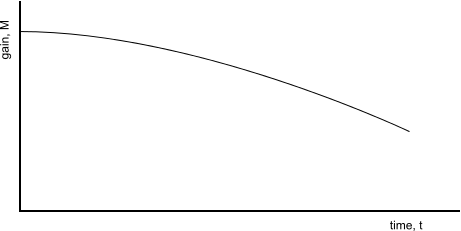
\includegraphics[width=0.7\textwidth, keepaspectratio=true]{chap2-Analog_Waveform.png}
  \caption{}
  \label{fig:chap2-Analog_Waveform}
\end{figure}

\begin{figure}[ht]
  \centering
    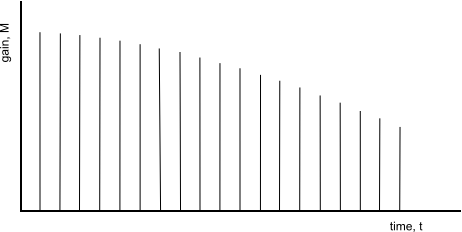
\includegraphics[width=0.7\textwidth, keepaspectratio=true]{chap2-Sampled_Waveform.png}
  \caption{}
  \label{fig:chap2-Sampled_Waveform}
\end{figure}

\section{ADC and DAC}\cite{smith1997dspbook}
Most of the signals directly encountered in science and engineering are continuous: light intensity that changes with distance; voltage that varies over time; etc. Analog-to-Digital Conversion (ADC) and Digital-to-Analog Conversion (DAC) are the processes that allow digital computers to interact with these everyday signals. Digital information is different from its continuous counterpart in two important respects: it is sampled, and it is quantized. Both of these restrict how much information a digital signal can
contain. This chapter describes the sampling frequency, number of bits, and type of analog filtering needed for converting between the analog and digital.

\begin{compactitem}
\item \textbf{Quantization}
Quantization is the process of representing the analog voltage from the sample-and-hold circuit by a fixed number of bits. The input analog voltage (or current) is compared to a set of pre-defined voltage (or current) levels. Each of the levels is represented by a unique binary number, and the binary number that corresponds to the level that is closest to the analog voltage is chosen to represent that sample. This process rounds the analog voltage to the nearest level, which means that the digital representation is an approximation to the analog voltage. There are a few methods for quantizing samples. The most commonly used ones are the dual slope method and the successive approximation.

\begin{figure}[ht]
  \centering
    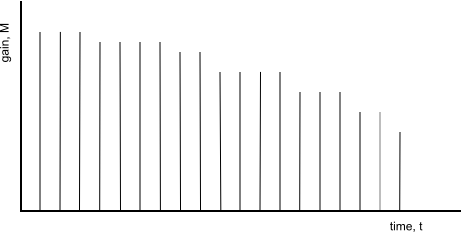
\includegraphics[width=0.7\textwidth, keepaspectratio=true]{chap2-Digital_Waveform.png}
  \caption{}
  \label{fig:chap2-Digital_Waveform}
\end{figure}


\item \textbf{The Sampling Theorem}\cite{dsp-nyquist}\\
The sampling theorem states that for a limited bandwidth (band-limited) signal with maximum frequency $f_{max}$, the equally spaced sampling frequency $f_s$ must be greater than twice of the maximum frequency $f_{max}$, i.e.,
$f_s > 2·f_{max}$
in order to have the signal be uniquely reconstructed without aliasing.

The frequency $2·f_{max}$ is called the \textbf{Nyquist sampling rate}. Half of this value, $f_{max}$, is sometimes called the \textbf{Nyquist frequency}.

\end{compactitem}

\section{Fourier Transform} \cite{csulb-Woollett}

\begin{compactitem}

\item {Fourier Series Expansion of a Function over $(-\boldsymbol{\pi,\,\pi})$}\\
A Fourier series expansion designed to represent a given function
  \textbf{f(x)} defined over a finite interval $(-\boldsymbol{\pi, \pi})$, is a sum of terms
\begin{equation}  \label{fxpi}
\mathbf{f(x) = \frac{1}{2} \, a_{0} + \sum_{n=1}^{\infty} \left[
   a_{n}\,\boldsymbol{\cos} (n\,x) + b_{n} \,\boldsymbol{\sin} (n\,x) \right] }
\end{equation}

\noindent and the constant coefficients ($\mathbf{a_{n},\, b_{n}}$) are
\begin{equation} \label{fcoeff}
 \mathbf{ a_{n} = \frac{1}{\boldsymbol{\pi}} \, \int_{-\boldsymbol{\pi}}^{\boldsymbol{\pi}} f(y)\,
   \boldsymbol{\cos} (n\,y) \, dy}, \quad
   \mathbf{ b_{n} = \frac{1}{\boldsymbol{\pi}} \, \int_{-\boldsymbol{\pi}}^{\boldsymbol{\pi}} f(y)\,
   \boldsymbol{\sin} (n\,y) \, dy}.
\end{equation}
(For a derivation of these equations see Sec.\ref{expfs} and Eqs.(\ref{Eq:piex1}) and
  (\ref{Eq:piex2}).)\\

\noindent The first term of the expansion
\begin{equation}
\mathbf{ \frac{1}{2} \, a_0  =
 \frac{1}{2\, \boldsymbol{\pi}}  \int_{-\boldsymbol{\pi}}^{\boldsymbol{\pi}} f(y)\,dy =
 \langle f(x) \rangle }
\end{equation}
is the (un-weighted) average of \textbf{f(x)} over the domain $(-\boldsymbol{\pi},\boldsymbol{\pi})$.
Hence $\mathbf{a_{0}}$ will always be twice the average value of the function over
  the domain.\\

\noindent If \textbf{f(x)} is an even function ($\mathbf{f(-x) =  f(x)}$),
  then only the $\mathbf{\boldsymbol{\cos}(n\,x)}$ terms
  contribute.
If \textbf{f(x)} is an odd function ($\mathbf{f(-x) =  -f(x)}$),
  then only the $\mathbf{\boldsymbol{\sin}(n\,x)}$ terms contribute. \\


\item {Fourier Transform}\\
\textbf{Fourier Cosine Integrals}
Given some function $\mathbf{f(x)}$ defined for $\mathbf{x \geq 0}$,
  we define the Fourier cosine transform  of this function as
\begin{equation}  \label{Eq:fc1}
\mathbf{F_{C}(f,\boldsymbol{\omega}) = \frac{2}{\boldsymbol{\pi}}
  \int_{0}^{\infty} \boldsymbol{\cos}(\boldsymbol{\omega}\,x)\,f(x)\,dx }
\end{equation}
The given function $\mathbf{f(x)}$ can then be written as an integral
  over positive values of $\boldsymbol{\omega}$:
\begin{equation}  \label{Eq:fc2}
\mathbf{f(x) = \int_{0}^{\infty} F_{C}(f,\boldsymbol{\omega})\,
    \cos(\boldsymbol{\omega}\,x)\,d\boldsymbol{\omega} }
\end{equation}
The two equations (\ref{Eq:fc1}) and (\ref{Eq:fc2}) are an example of
  a "Fourier transform pair", which include conventions about where
  to place the factor of $2/\boldsymbol{\pi}$.\\

\textbf{Fourier Sine Integrals}\\
Given some function $\mathbf{f(x)}$ defined for $\mathbf{x \geq 0}$,
  we define the Fourier sine transform  of this function as
\begin{equation}  \label{Eq:fsine1}
\mathbf{F_{S}(f,\boldsymbol{\omega}) = \frac{2}{\boldsymbol{\pi}}
  \int_{0}^{\infty} \boldsymbol{\sin}(\boldsymbol{\omega}\,x)\,f(x)\,dx }
\end{equation}
The given function $\mathbf{f(x)}$ can then be written as an integral
  over positive values of $\boldsymbol{\omega}$:
\begin{equation}  \label{Eq:fsine2}
\mathbf{f(x) = \int_{0}^{\infty} F_{S}(f,\boldsymbol{\omega})\,
    \sin(\boldsymbol{\omega}\,x)\,d\boldsymbol{\omega} }
\end{equation}
The two equations (\ref{Eq:fsine1}) and (\ref{Eq:fsine2}) are another
   "Fourier transform pair", which include conventions about where
  to place the factor of $2/\boldsymbol{\pi}$.

\textbf{Exponential Fourier Integrals}\\
Given some function $\mathbf{f(x)}$ defined for $\mathbf{-\infty <x < \infty}$,
  we define the exponential Fourier transform  of this function as
\begin{equation}  \label{Eq:fexp1}
\mathbf{F_{Exp}(f,\boldsymbol{\omega}) = \frac{1}{2\, \boldsymbol{\pi}}
  \int_{-\infty}^{\infty} \,f(x) e^{i\,\boldsymbol{\omega}\,x}\,dx }
\end{equation}
The given function $\mathbf{f(x)}$ can then be written as an integral
  over both positive and negative values of $\boldsymbol{\omega}$:
\begin{equation}  \label{Eq:fexp2}
\mathbf{f(x) = \int_{-\infty}^{\infty} F_{Exp}(f,\boldsymbol{\omega})\,
    e^{-i\,\boldsymbol{\omega}\,x} \,d\boldsymbol{\omega} }
\end{equation}
The two equations (\ref{Eq:fexp1}) and (\ref{Eq:fexp2}) are another
   "Fourier transform pair", which include conventions about where
  to place the factor of $\mathbf{2\, \boldsymbol{\pi}}$ as well as which member
  has the minus sign in the exponent.\\

\noindent If the given function is even, $\mathbf{f(-x) = f(x) }$, then the
exponential Fourier transform has the symmetry
\begin{equation}
\mathbf{F_{Exp}(f,\boldsymbol{-\omega}) = F_{Exp}(f,\boldsymbol{\omega}) }
\end{equation}
and can be expressed in terms of the Fourier cosine transform:
\begin{equation}
\mathbf{F_{Exp}(f,\boldsymbol{\omega}) = \frac{1}{2} \, F_{C}(f,\boldsymbol{\omega})}.
\end{equation}
If the given function is odd, $\mathbf{f(-x) = -f(x) }$, then the
exponential Fourier transform has the symmetry
\begin{equation}
\mathbf{F_{Exp}(f,\boldsymbol{-\omega}) = -F_{Exp}(f,\boldsymbol{\omega}) }
\end{equation}
and can be expressed in terms of the Fourier sine transform:
\begin{equation}
\mathbf{F_{Exp}(f,\boldsymbol{\omega}) = \frac{i}{2} \, F_{S}(f,\boldsymbol{\omega})}.
\end{equation}
If the given function is neither even nor odd, the function can always be written
  as the sum of an even function $\mathbf{f_{e}(x)}$ and an odd function $\mathbf{f_{o}(x)}$:
\begin{equation}
\mathbf{f(x) \equiv f_{e}(x) + f_{o}(x) =
  \frac{1}{2} \,( f(x) + f(-x) + \frac{1}{2} \, ( f(x) - f(-x) }
\end{equation}
and can be expressed in terms of the Fourier cosine transform of $\mathbf{f_{e}(x)}$
  and the Fourier sine transform of $\mathbf{f_{o}(x)}$:
\begin{equation}
\mathbf{F_{Exp}(f,\boldsymbol{\omega}) \equiv F_{Exp}(f_{e}+f_{o},\boldsymbol{\omega}) =
  \frac{1}{2} \, F_{C}(f_{e},\boldsymbol{\omega}) +
  \frac{i}{2} \, F_{S}(f_{o},\boldsymbol{\omega}) }
\end{equation}


\item {Discrete Fourier Transform}

\begin{figure}[ht]
  \label{fig:chap2-DFT}
  \centering
	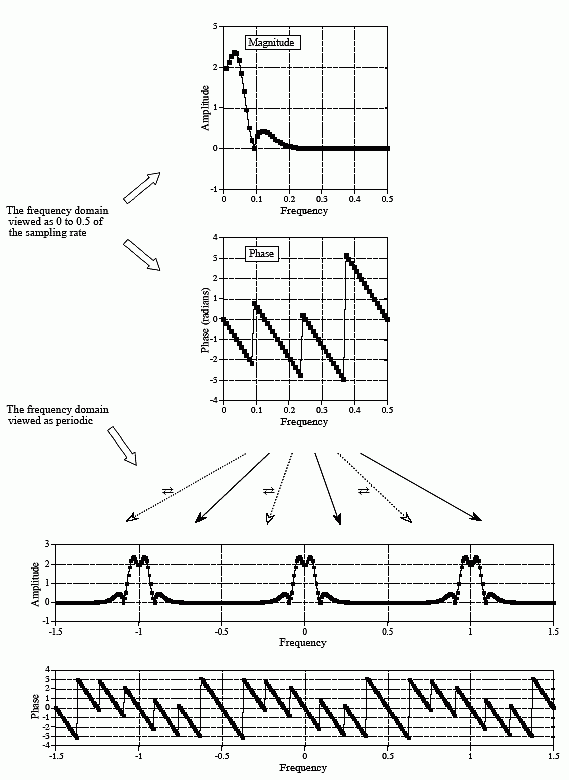
\includegraphics[width=0.7\textwidth, keepaspectratio=true]{chap2-DFT.png}
	\caption{}
\end{figure}\cite{smith1997scientist}

\item {Fast Fourier Transform}
\begin{figure}
  \label{fig:chap2-FFT}
  \centering
	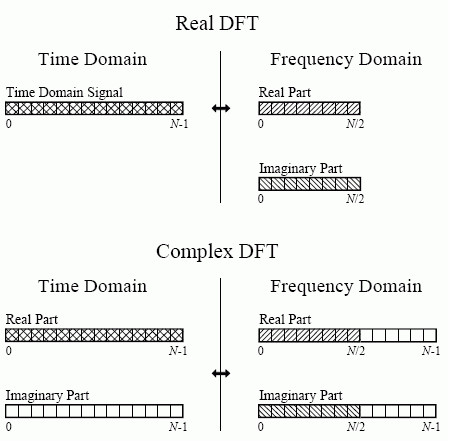
\includegraphics[width=\textwidth, keepaspectratio=true]{chap2-FFT.png}
\caption{Comparing the \textbf{real} and \textbf{complex} DFTs.
The real DFT takes an \textbf{N point} time domain signal and creates \textbf{two N/2-1} point frequency domain %signals. The \textbf{complex DFT} takes two N point time domain signals and creates two N point frequency domain signals. The crosshatched regions shows
the values common to the two transforms.}
\end{figure}


The \textbf{FFT} is based on the \textbf{complex DFT}.
Since the FFT is an algorithm for calculating the complex DFT. \autoref{chap2-FFT}
compares how the real DFT and the complex DFT store data.\\

The \textbf{real DFT} transforms an \textbf{N point} time domain signal into
\textbf{two N/2} + 1 point frequency domain signals. The time domain
signal is called just that: the \textbf{time domain signal}. The two signals in the
\textbf{frequency domain} are called the \textbf{real part} and the \textbf{imaginary part},
holding the \textbf{amplitudes of the cosine waves and sine waves}, respectively.
In comparison, the \textbf{complex DFT transforms} \textbf{two N point} time domain signals
into \textbf{two N point} frequency domain signals. The two time domain signals are
called the \textbf{real part} and the \textbf{imaginary part}, just as are the frequency domain
signals.
\\Suppose you have \textbf{an N point} signal, and need to calculate the \textbf{real DFT} by
means of the \textbf{Complex DFT} (such as by using the FFT algorithm).\\
\textbf{First}, move the \textbf{N point} signal into the \textbf{real part} of the \textbf{complex DFT's} time domain.\\
\textbf{Second}, set all of the samples in the \textbf{imaginary} part to \textbf{zero}.\\
\textbf{Third}, calculation of the \textbf{complex DFT} results in a \textbf{real} and an \textbf{imaginary}
signal in the frequency domain, each composed of \textbf{N} points.
Samples 0 through N/2 of these signals correspond to the \textbf{real DFT's} spectrum.\\
The complex DFT's frequency spectrum includes the negative frequencies in the 0
to 1.0 arrangement. In other words, one full period stretches from sample 0 to
sample N-1 , corresponding with 0 to 1.0 times the sampling rate. The positive
frequencies sit between sample 0 and N/2 , corresponding with 0 to 0.5. The
other samples, between N/2 + 1 and N-1 , contain the negative frequency
values (which are usually ignored). \cite{smith1997dspbook}

%\item {Power Spectra}

\end{compactitem}

%----------------------------------------------------------------------------------------

\section{ICA}
Independent Component Analysis (ICA) is a computationally efficient blind source separation technique.
It has been an area of interest for researchers for many practical applications in various fields of science and
engineering.

\cite{journals/informaticaSI/NaikK11}
\begin{compactitem}

\item {Introduction}
The problem of source separation is an inductive inference problem. There is not enough information
to deduce the solution, so one must use any available information to infer the most probable solution.
The problem of separating and estimating the original source waveforms from the sensor array,
without knowing the transmission channel characteristics and the source can be briefly expressed
as problems related to BSS. In BSS the word blind refers to the fact that we do not know how the signals
were mixed or how they were generated. As such, the separation is in principle impossible. Allowing some relatively indirect and general constrains, we however still hold the term BSS valid, and separate under these conditions. There appears to be something magical about blind source separation; we are estimating the original source signals without knowing the parameters of mixing and/orfiltering processes. Independent component analysis (ICA) is one of the most widely used BSS techniques for revealing hidden factors that underlie sets of random variables, measurements, or signals. ICA is essentially a method for extracting individual
signals from mixtures. Its power resides in the physical assumptions that the different physical processes
generate unrelated signals. The simple and generic nature of this assumption allows ICA to be successfully applied in diverse range of research fields. The BSS is unsupervised and thought of as a black box method.

\item {ICA model}
The general model for ICA is that the sources are generated
through a linear basis transformation, where additive
noise can be present. Suppose we have N statistically independent
signals, si(t), i = 1, ...,N. We assume that the
sources themselves cannot be directly observed and that
each signal, si(t), is a realization of some fixed probability
distribution at each time point t. Also, suppose we observe
these signals using N sensors, then we obtain a set of N observation
signals xi(t), i = 1, ...,N that are mixtures of the
sources. A fundamental aspect of the mixing process is that
the sensors must be spatially separated (e.g. microphones
that are spatially distributed around a room) so that each
sensor records a different mixture of the sources. With this
spatial separation assumption in mind, we can model the
mixing process with matrix multiplication as follows:

\begin{equation}
\label{eq:ica-linear}
\\
x(t) = As(t)
\end{equation}\\

where A is an unknown matrix called the mixing matrix
and $x(t), s(t)$ are the two vectors representing the observed
signals and source signals respectively. Incidentally, the
justification for the description of this signal processing
technique as blind is that we have no information on the
mixing matrix, or even on the sources themselves.
The objective is to recover the original signals, $s_i(t)$,
from only the observed vector $x_i(t)$. We obtain estimates
for the sources by first obtaining the “unmixing matrix” $W$,
where,
This enables an estimate, $\hat{s}(t)$, of the independent
sources to be obtained:

\begin{equation}
\label{eq:ica-white}
\hat{s}(t) =Wx(t)
\end{equation}\\

The diagram in Figure 1 illustrates both the mixing
and unmixing process involved in BSS. The independent
sources are mixed by the matrix A (which is unknown in
this case). We seek to obtain a vector y that approximates
s by estimating the unmixing matrix W. If the estimate of
the unmixing matrix is accurate, we obtain a good approximation
of the sources.
The above described ICA model is the simple model
since it ignores all noise components and any time delay
in the recordings.
\item {Independence}

A key concept that constitutes the foundation of independent
component analysis is statistical independence. To
simplify the above discussion consider the case of two different
random variables s1 and s2. The random variable s1
is independent of s2, if the information about the value of
s1 does not provide any information about the value of s2,
and vice versa. Here s1 and s2 could be random signals
originating from two different physical process that are not
related to each other.

\begin{figure}[ht]
  \centering
    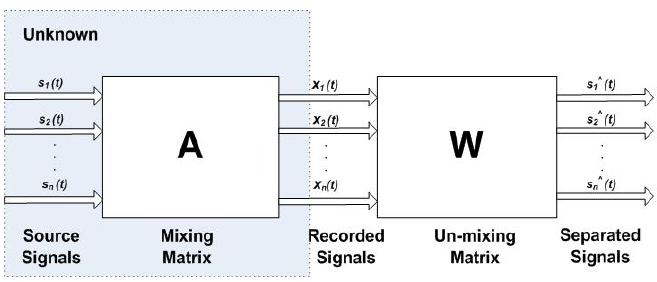
\includegraphics[width=0.7\textwidth, keepaspectratio=true]{chap2-ICA.png}
  \caption{Blind source separation (BSS) block diagram. $s(t)$ are the sources. $x(t)$ are the recordings,
	$\hat{s}(t)$ are the estimated sources A is mixing matrix and W is un-mixing matrix. }
  \label{fig:chap2-ICA}
\end{figure}

\item {Preprocessing}
Before examining specific ICA algorithms, it is instructive
to discuss preprocessing steps that are generally carried out
before ICA.

\item {Centering}
A simple preprocessing step that is commonly performed
is to “center” the observation vector x by subtracting its
mean vector $m=E{x}$. That is then we obtain the centered
observation vector, $x_c$, as follows:
\begin{equation}
\label{eq:ica-zero-mean}
x_c = x-m
\end{equation}

This step simplifies ICA algorithms by allowing us to
assume a zero mean. Once the unmixing matrix has been
estimated using the centered data, we can obtain the actual
estimates of the independent components as follows:

\begin{equation}
\label{eq:ica-source}
\hat{s}(t) = A^{-1} (x_c + m )
\end{equation}

From this point on, all observation vectors will be assumed
centered. The mixing matrix, on the other hand,
remains the same after this preprocessing, so we can always
do this without affecting the estimation of the mixing
matrix.

\item {Whitening}
Another step which is very useful in practice is to prewhiten
the observation vector x. Whitening involves linearly
transforming the observation vector such that its components
are uncorrelated and have unit variance . Let
xw denote the whitened vector, then it satisfies the following
equation:
\begin{equation}
\label{eq:ica-source1}
E{x_w x^T_w} = I
\end{equation}

where $E{x_w x^T_w}$ is the covariance matrix of $x_w$. Also,
since the ICA framework is insensitive to the variances
of the independent components, we can assume without
loss of generality that the source vector, s, is white, i.e.
$E{s s^T } = I$
A simple method to perform the whitening transformation
is to use the eigenvalue decomposition (EVD) of x.
That is, we decompose the covariance matrix of x as follows:
\begin{equation}
\label{eq:ica-evd}
E{x x^T } =VDV^T
\end{equation}
where V is the matrix of eigenvectors of $E{x x^T }$,
and D is the diagonal matrix of eigenvalues, i.e.
$D = diag{\lambda_1,\lambda_2, ...,\lambda_n}$. The observation vector can be
whitened by the following transformation:
\begin{equation}
\label{eq:ica-whiteningX1}
x_w = VD^{-1/2}V^Tx
\end{equation}
where the matrix $D^{-1/2}$ is obtained by a
simple component wise operation as $D^{-1/2}=diag{\lambda_1^{-1/2},\lambda_2^{-1/2},...,\lambda_n^{-1/2}}$. Whitening transforms
the mixing matrix into a new one, which is orthogonal
\begin{equation}
\label{eq:ica-whiteningX}
x_w=VD^(-1/2)V^TAs=A_w s
\end{equation}

hence,
\begin{equation}
\label{eq:ica-CoVI}
E{x_w x^T_w } = A_w E{s s^T }A^T_w
= A_w A^T_w = I
\end{equation}

Whitening thus reduces the number of parameters to be
estimated. Instead of having to estimate the $n^2$ elements of
the original matrix A, we only need to estimate the new orthogonal
mixing matrix, where An orthogonal matrix has
$n(n-1)/2$ degrees of freedom. One can say that whitening
solves half of the ICA problem. This is a very useful step
as whitening is a simple and efficient process that significantly
reduces the computational complexity of ICA. An illustration
of the whitening process with simple ICA source
separation process is explained in the later section.

\item {ICA Algorithms}
There are several ICA algorithms available in literature.
However the following algorithms are widely used
in numerous signal processing applications. These includes
FastICA, JADE, and ICA RADICAL. Each algorithm used a different
approach to solve equation. We will use ICA RADICAL \cite{radical-ica} to solve our PPG problem.

\end{compactitem}


%% Chapter 4
\chapter{Machine Learning} % Main chapter title

\label{Chapter4} % For referencing the chapter elsewhere, use \ref{Chapter1} 

\lhead{Chapter 4. \emph{Machine Learning}} % This is for the header on each page - perhaps a shortened title

%----------------------------------------------------------------------------------------
\section{Decision Tree}
\section{Ensemble Learning}
\section{Random Forest}
\section{Adaboost}

\begin{compactitem}

\item Diagonal Matrix Properties
In linear algebra, a diagonal matrix is a matrix (usually a square matrix) in which 
the entries outside the main diagonal are all zero. The diagonal entries themselves 
may or may not be zero. Thus, the matrix $D = (d_{i,j})$ with n columns and n rows is diagonal 
The time complexity is $O(N^2),  (C_2^N) = O(N^2/2)$.
\end{compactitem}

%----------------------------------------------------------------------------------------

\section{In Closing}

You have reached the end of this mini-guide. You can now rename or overwrite this pdf file and begin writing your own `\texttt{Chapter1.tex}' and the rest of your thesis. The easy work of setting up the structure and framework has been taken care of for you. It's now your job to fill it out!

Good luck and have lots of fun!

\begin{flushright}
Guide written by ---\\
Sunil Patel: \href{http://www.sunilpatel.co.uk}{www.sunilpatel.co.uk}
\end{flushright}

%% Chapter 4
\chapter{Face Detection} % Main chapter title

\label{Chapter4} % For referencing the chapter elsewhere, use \ref{Chapter1}

\lhead{Chapter 4. \emph{Face Detection}} % This is for the header on each page - perhaps a shortened title

A face detector has to tell whether an image of arbitrary size contains a human face and if so, where
it is. One natural framework for considering this problem is that of binary classification, in which
a classifier is constructed to minimize the misclassification risk. Since no objective distribution can
describe the actual prior probability for a given image to have a face, the algorithm must minimize
both the false negative and false positive rates in order to achieve an acceptable performance.
This task requires an accurate numerical description of what sets human faces apart from other
objects. It turns out that these characteristics can be extracted with a remarkable committee learning
algorithm called Adaboost, which relies on a committee of weak classifiers to form a strong
one through a voting mechanism. An operational algorithm must also work with a reasonable computational 
budget. Techniques such as integral image and attentional cascade make the Viola-Jones algorithm \cite{Viola2004RRF966432}
highly efficient: fed with a real time image sequence generated from a standard webcam, it performs well on a
standard PC.\cite{ipol.2014.104}

%----------------------------------------------------------------------------------------
\section{Robust Real-time Object Detection}
The Viola-Jones algorithm  \cite{Viola2004RRF966432}, the first ever real-time face detection system. 
There are three contributions of Viola-Jones algorithm to enable a fast and accurate detection:
the \textbf{integral image} for feature computation, \textbf{Adaboost} for feature selection and an 
\textbf{attentional cascade} for efficient computational resource allocation. 
Since the Viola-Jones algorithm typically gives multiple detections, 
a post-processing step is also proposed to reduce detection redundancy using a robustness argument.\cite{ipol.2014.104}


\begin{compactitem}
\item {Features}
The Viola-Jones object detection procedure classifies images based on the value of simple features.
There are many motivations for using features rather than the pixels directly. The feature-based system 
operates much faster than a pixel-based system.
The simple features used are Haar basis functions. There are three kinds of features used. 
The value of a two-rectangle feature is the difference between the sum of the pixels within
two rectangular regions. The regions have the same size and shape and are horizontally
or vertically adjacent (see \autoref{fig:chap4-Haar}). A three-rectangle feature computes the sum within
two outside rectangles subtracted from the sum in a center rectangle. Finally a fourrectangle
feature computes the difference between diagonal pairs of rectangles.
Given that the base resolution of the detector is 24x24, the exhaustive set of rectangle
features is quite large, 45,396.

\begin{figure}[h]
  \centering
	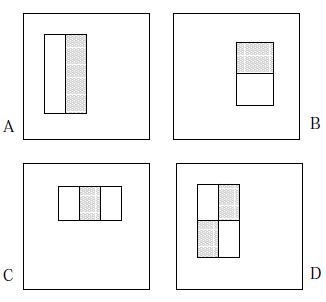
\includegraphics[width=0.7\textwidth, keepaspectratio=true]{chap4-Haar.png}
  \caption{Example rectangle features shown relative to the enclosing detection window.
The sum of the pixels which lie within the white rectangles are subtracted from the
sum of pixels in the grey rectangles. Two-rectangle features are shown in (A) and (B).
Figure (C) shows a three-rectangle feature, and (D) a four-rectangle feature.}
  \label{fig:chap4-Haar}
\end{figure}

\item {Integral Image}
Rectangle features can be computed very rapidly using an intermediate representation
for the image which we call the integral image. The integral image at location x, y
contains the sum of the pixels above and to the left of x, y, inclusive:
$ii(x; y) = X x0x;y0yi(x0; y0);$
where $ii(x, y)$ is the integral image and $i(x, y)$ is the original image (see \autoref{fig:chap4-Integral}).
Using the following pair of recurrences:
%s(x; y) = s(x; y 􀀀 1) + i(x; y) (1)
%ii(x; y) = ii(x 􀀀 1; y) + s(x; y) (2)
%(where s(x; y) is the cumulative row sum, s(x;􀀀1) = 0, and ii(􀀀1; y) = 0) the
integral image can be computed in one pass over the original image.
Using the integral image any rectangular sum can be computed in four array references
(see  \autoref{fig:chap4-Integral4}). Clearly the difference between two rectangular sums can be
computed in eight references. Since the two-rectangle features defined above involve
adjacent rectangular sums they can be computed in six array references, eight in the
case of the three-rectangle features, and nine for four-rectangle features.
One alternative motivation for the integral image comes from the “boxlets” work
of Simard, et al.
\begin{figure}[h]
  \centering
	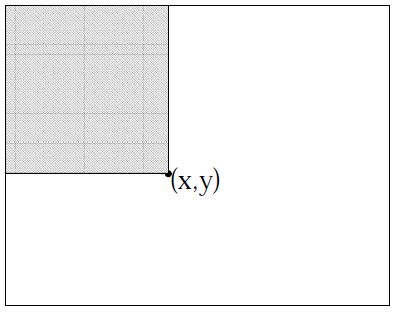
\includegraphics[width=0.7\textwidth, keepaspectratio=true]{chap4-Integral.png}
  \caption{The value of the integral image at point (x; y) is the sum of all the pixels
above and to the left.}
  \label{fig:chap4-Integral}
\end{figure}

\begin{figure}[h]
  \centering
	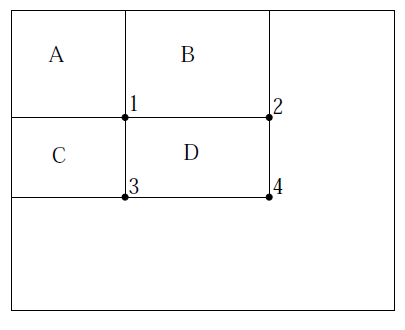
\includegraphics[width=0.7\textwidth, keepaspectratio=true]{chap4-Integral4.png}
  \caption{The sum of the pixels within rectangle D can be computed with four array
references. The value of the integral image at location 1 is the sum of the pixels in
rectangle A. The value at location 2 is A + B, at location 3 is A + C, and at location
4 is A + B + C + D. The sum within D can be computed as 4 + 1 - (2 + 3)}
  \label{fig:chap4-Integral4}
\end{figure}


\item {Feature Selection with Adaboost}
\item {The Attentional Cascade}
This section describes an algorithm for constructing a cascade of classifiers which
achieves increased detection performance while radically reducing computation time.
The key insight is that smaller, and therefore more efficient, boosted classifiers can be
constructed which reject many of the negative sub-windows while detecting almost all
positive instances. Simpler classifiers are used to reject the majority of sub-windows
before more complex classifiers are called upon to achieve low false positive rates.
Stages in the cascade are constructed by training classifiers using AdaBoost. Starting
with a two-feature strong classifier, an effective face filter can be obtained by adjusting
the strong classifier threshold to minimize false negatives. The initial AdaBoost
threshold, 
%1
%2 PT t=1 t, 
is designed to yield a low error rate on the training data. A lower
threshold yields higher detection rates and higher false positive rates. Based on performance
measured using a validation training set, the two-feature classifier can be
adjusted to detect 100% of the faces with a false positive rate of 40%. See Figure 5 for
a description of the two features used in this classifier.
The detection performance of the two-feature classifier is far from acceptable as an
object detection system. Nevertheless the classifier can significantly reduce the number
of sub-windows that need further processing with very few operations:
1. Evaluate the rectangle features (requires between 6 and 9 array references per
feature).
2. Compute the weak classifier for each feature (requires one threshold operation
per feature).
3. Combine the weak classifiers (requires one multiply per feature, an addition, and
finally a threshold).
A two feature classifier amounts to about 60 microprocessor instructions. It seems
hard to imagine that any simpler filter could achieve higher rejection rates. By comparison,
scanning a simple image template, or a single layer perceptron, would require at
least 20 times as many operations per sub-window.
The overall form of the detection process is that of a degenerate decision tree, what
we call a “cascade” [9] (see Figure 6). A positive result from the first classifier triggers
the evaluation of a second classifier which has also been adjusted to achieve very high
detection rates. A positive result from the second classifier triggers a third classifier,
and so on. A negative outcome at any point leads to the immediate rejection of the
sub-window.
The structure of the cascade reflects the fact that within any single image an overwhelming
majority of sub-windows are negative. As such, the cascade attempts to
reject as many negatives as possible at the earliest stage possible. While a positive
instance will trigger the evaluation of every classifier in the cascade, this is an exceedingly
rare event.
Much like a decision tree, subsequent classifiers are trained using those examples
which pass through all the previous stages. As a result, the second classifier faces a
more difficult task than the first. The examples which make it through the first stage are
“harder” than typical examples. The more difficult examples faced by deeper classifiers
push the entire reciever operating characteristic (ROC) curve downward. At a given
detection rate, deeper classifiers have correspondingly higher false positive rates.

\begin{figure}[h]
  \centering
	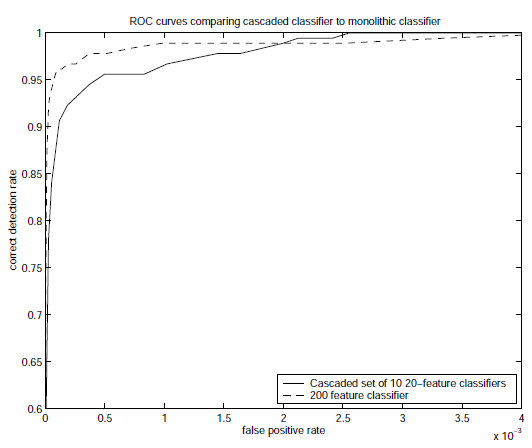
\includegraphics[width=0.7\textwidth, keepaspectratio=true]{chap4-ROC.png}
  \caption{Reciever operating characteristic (ROC) curve for the 200 feature classifier.}
  \label{fig:chap4-ROC}
\end{figure}

\begin{figure}[h]
  \centering
	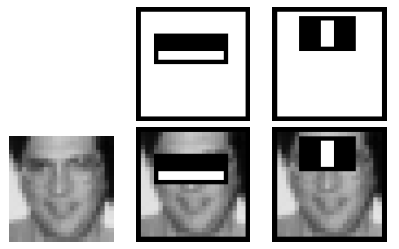
\includegraphics[width=0.7\textwidth, keepaspectratio=true]{chap4-Face.png}
  \caption{The first and second features selected by AdaBoost. The two features are
shown in the top row and then overlayed on a typical training face in the bottom row.
The first feature measures the difference in intensity between the region of the eyes and
a region across the upper cheeks. The feature capitalizes on the observation that the
eye region is often darker than the cheeks. The second feature compares the intensities
in the eye regions to the intensity across the bridge of the nose}
  \label{fig:chap4-Face}
\end{figure}


\begin{figure}[h]
  \centering
	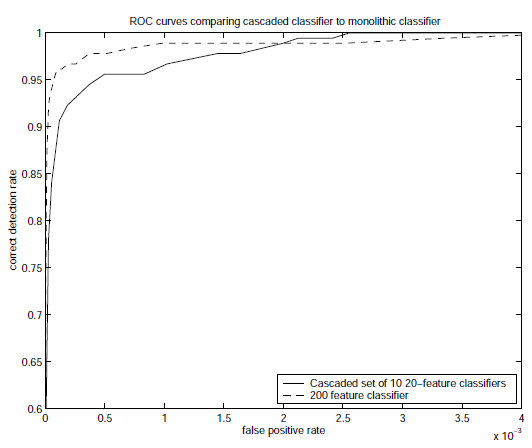
\includegraphics[width=0.7\textwidth, keepaspectratio=true]{chap4-Cascade.png}
  \caption{Schematic depiction of a the detection cascade. A series of classifiers are applied
to every sub-window. The initial classifier eliminates a large number of negative
examples with very little processing. Subsequent layers eliminate additional negatives
but require additional computation. After several stages of processing the number of
sub-windows have been reduced radically. Further processing can take any form such
as additional stages of the cascade (as in our detection system) or an alternative detection
system..}
  \label{fig:chap4-Cascade}
\end{figure}

\end{compactitem}

\section{PICO}
Object Detection with Pixel Intensity Comparisons Organized in Decision Trees
\cite{DBLPjournalscorrabs}

\section{NPD}

%----------------------------------------------------------------------------------------


%% Chapter 5
\chapter{Multispectral Human Skin Detection}% Main chapter title

\label{Chapter5} % For referencing the chapter elsewhere, use \ref{Chapter1}

\lhead{Chapter 5. \emph{Multispectral}} % This is for the header on each page - perhaps a shortened title

%----------------------------------------------------------------------------------------
\section{Introduction}
The conventional methods for detecting objects, which employ pattern
recognition, have many problems, for example, an increase in processing time,
a difficulty of detecting occluded objects, a necessity of huge data for machine
learning and so on. To overcome these problems, a method for detecting human skin
that employs a spectroscopic camera will be studied. Each substance has its
own reflection characteristics. In particular, human
skin reflects flesh-colored light in the visible region and
absorbs light with a wavelength of 970 nm. Thus, to detect human skin,
a multi-band camera that has red, green, blue, 870, 970, and 1050 nm filters will be
studied. By using this multi-band camera, human
skin in Y Cr Cb color space around the visible region
and dips around 970 nm in the near-infrared region is detected. \cite{Kanzawa_humanskin}

\begin{figure}[ht]
  \centering
    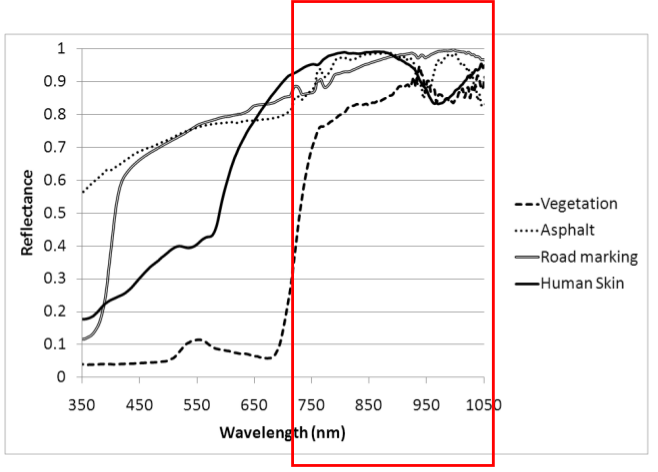
\includegraphics[width=0.7\textwidth, keepaspectratio=true]{chap6-Reflectance.png}
  \caption{Reflectance spectra of various substances.}
  \label{fig:chap6_Reflectance}
\end{figure}

\section {Reflectance Spectrum of Human Skin}
Spectroscopy is the study of how substances absorb,
transmit, or reflect light. A conventional camera sensor
can obtain images in the ultraviolet (UV),
Vis, and NIR regions. UV–Vis–NIR spectroscopy is
applied for optical absorbance and reflectance measurements in the wavelength
range 200–1500 nm. Because a substance has its own unique reflectance
characteristics, we can distinguish a substance by analyzing the
light reflectance. Reflectance spectra of some substances, for example
asphalt, road markings and human skin are depicted in \autoref{fig:chap6_Reflectance}.
The horizontal and vertical axis show the wavelength and reflectance, respectively.

\autoref{fig:chap6_humanskin} shows only a reflectance spectrum of human
skin. Skin has a lower reflectance at shorter wavelengths (about 350 nm) than at
longer wavelengths (about 1050 nm). In particular, skin has a unique
property that it absorbs light around a wavelength of 970nm in the NIR region.
\begin{figure}[ht]
  \centering
    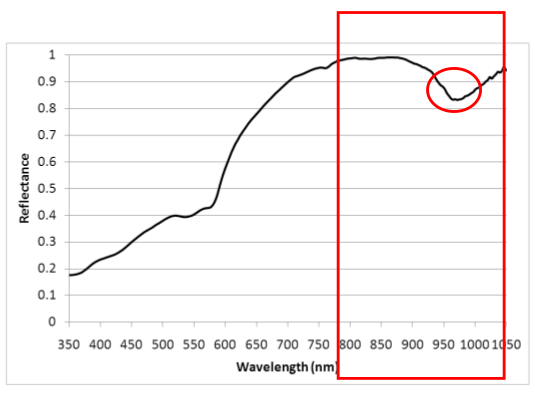
\includegraphics[width=0.7\textwidth, keepaspectratio=true]{chap6-humanskin.png}
  \caption{Reflectance spectra of human skin.}
  \label{fig:chap6_humanskin}
\end{figure}

The reflectance spectra of skin from about 50 people who have various
races are measured; all the spectra revealed that light was absorbed
at a wavelength of 970 nm, as shown in \autoref{fig:chap6_humanrace}.

\begin{figure}[ht]
  \centering
    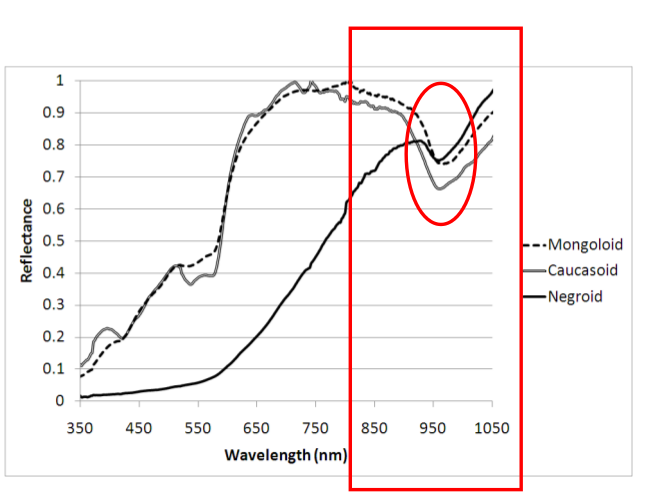
\includegraphics[width=0.7\textwidth, keepaspectratio=true]{chap6-humanrace.png}
  \caption{Spectra of various human skin.}
  \label{fig:chap6_humanrace}
\end{figure}

%----------------------------------------------------------------------------------------
\section{Multi-Camera Module}
Human skin reflects flesh-colored light in the Vis region and absorbs light
with a wavelength of 970 nm in the NIR region. A multi-band camera is studied to
exploit these characteristics. It has two types of cameras: a Vis camera that
acquires three images around Vis regions as a conventional color camera and
a NIR camera that can acquire three images in individual NIR wavelengths (870, 950,
1050nm). \autoref{fig:chap6_mcam} shows a photograph of the multi-band camera schematic.

\begin{figure}[hb]
  \centering
    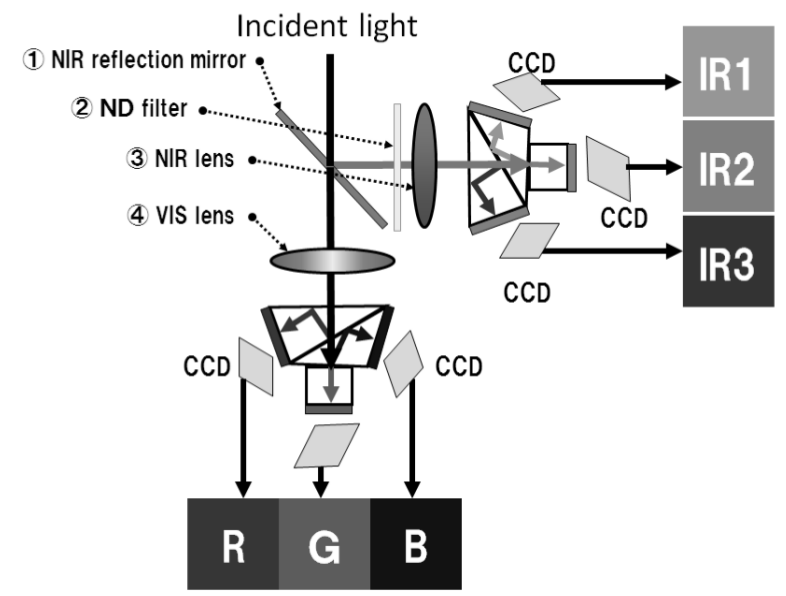
\includegraphics[width=0.7\textwidth, keepaspectratio=true]{chap6-mcam.png}
  \caption{Schematic diagram of the multi-camera module.}
  \label{fig:chap6_mcam}
\end{figure}
%----------------------------------------------------------------------------------------
\section {Human Skin Detection}
Conventionally, for detecting human skin from images,
visible color image processing methods are used.
However, it has been well known that color information is easily affected
from a change of illumination condition. A NIR image processing method is proposed
to detect human skin. This method is based on the characteristics of spectroscopy
around NIR region, therefore unaffected from visible
light. But, since clouds and water vapor absorbs light
with a wavelength of 940nm as shown in \autoref{fig:chap6_water},
it is difficult to distinguish human skin, which absorbs light with a wavelength
of 970nm, from clouds. To overcome above problems, a multi-band camera is studied.
Both visible color and NIR image processing methods are combined for detecting
human skin.

\begin{figure}[hb]
  \centering
	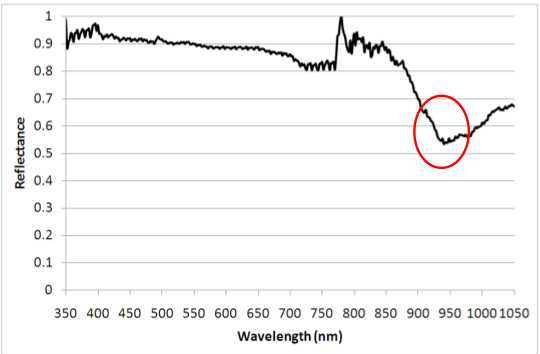
\includegraphics[width=0.7\textwidth, keepaspectratio=true]{chap6-water.png}
  \caption{Reflectance spectra of clouds and water vapor.}
  \label{fig:chap6_water}
\end{figure}

%% Chapter 6
\chapter{Motion-Robust and Ambient Light-Immune Remote PPG} % Main chapter title

\label{Chapter6} % For referencing the chapter elsewhere, use \ref{Chapter1}

\lhead{Chapter 6. \emph{Fundamental Mathematics}} % This is for the header on each page - perhaps a shortened title

%----------------------------------------------------------------------------------------
\section {Photoplethysmogram PPG \cite{wiki-PPG}}
\begin{figure}[hb]
  \centering
    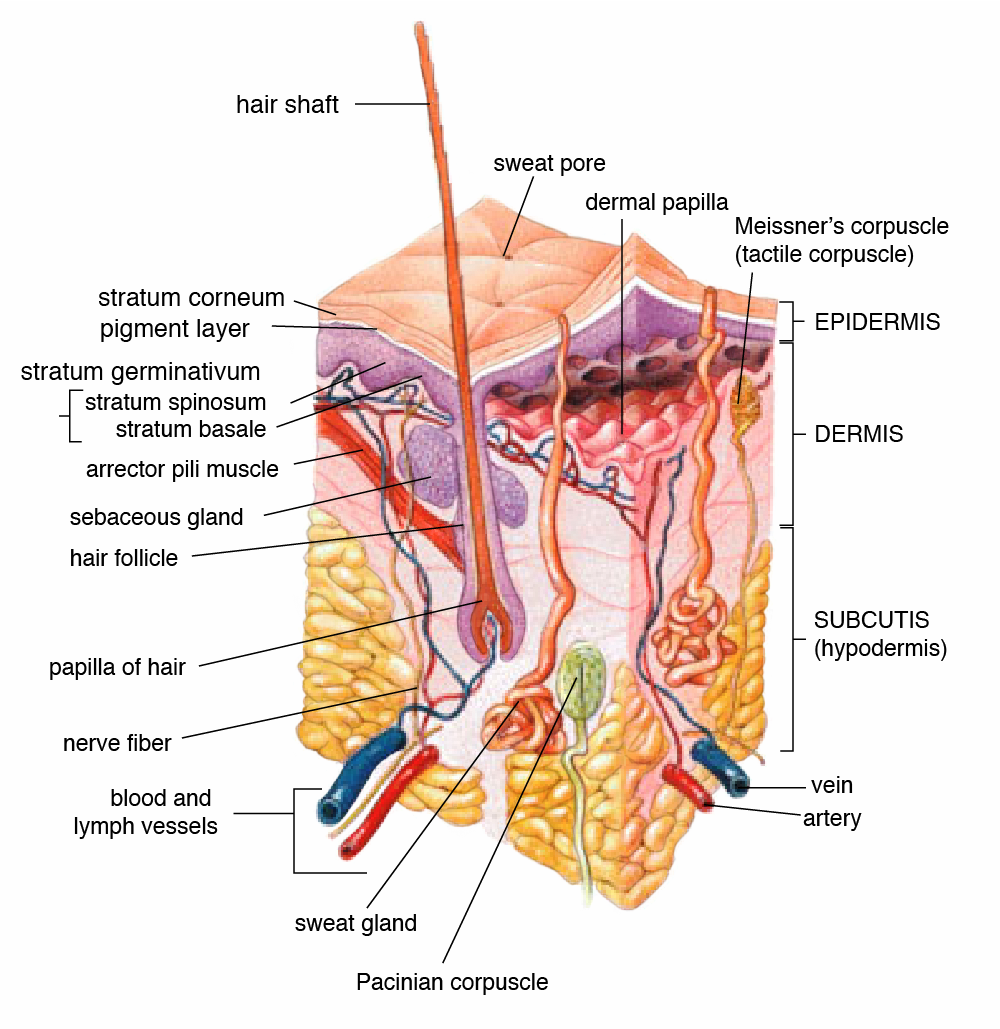
\includegraphics[width=0.7\textwidth, keepaspectratio=true]{chap6-Skinppg.png}
  \caption{Diagram of the layers of human skin.}
  \label{fig:chap6-Skinppg}
\end{figure}

A photoplethysmogram (PPG) is an optically obtained plethysmogram, a volumetric measurement of an organ.
A PPG is often obtained by using a pulse oximeter which illuminates the skin and measures changes in light absorption.
A conventional pulse oximeter monitors the perfusion of blood to the dermis and subcutaneous tissue of the skin.

Diagram of the layers of human skin \autoref{fig:chap6-Skinppg} With each cardiac cycle the heart pumps
blood to the periphery. Even though this pressure pulse is somewhat damped
by the time it reaches the skin, it is enough to distend the arteries and
arterioles in the subcutaneous tissue.

The change in volume caused by the pressure pulse is detected by illuminating the skin
with the light from a light-emitting diode (LED) and then measuring the amount of
light either transmitted or reflected to a photodiode.
Each cardiac cycle appears as a peak, as seen in the \autoref{fig:chap6-PVC}.
Because blood flow to the skin can be modulated by multiple other physiological systems,
the PPG can also be used to monitor breathing, hypovolemia,
and other circulatory conditions.

Sites for measuring PPG
While pulse oximeters are a commonly used medical device the PPG derived from them is
rarely displayed, and is nominally only processed to determine heart rate.
PPGs can be obtained from transmissive absorption (as at the finger tip) or
reflection (as on the forehead).

Motion artifacts have been shown to be a limiting factor preventing accurate readings
during exercise and free living conditions.
\begin{figure}[h]
  \centering
    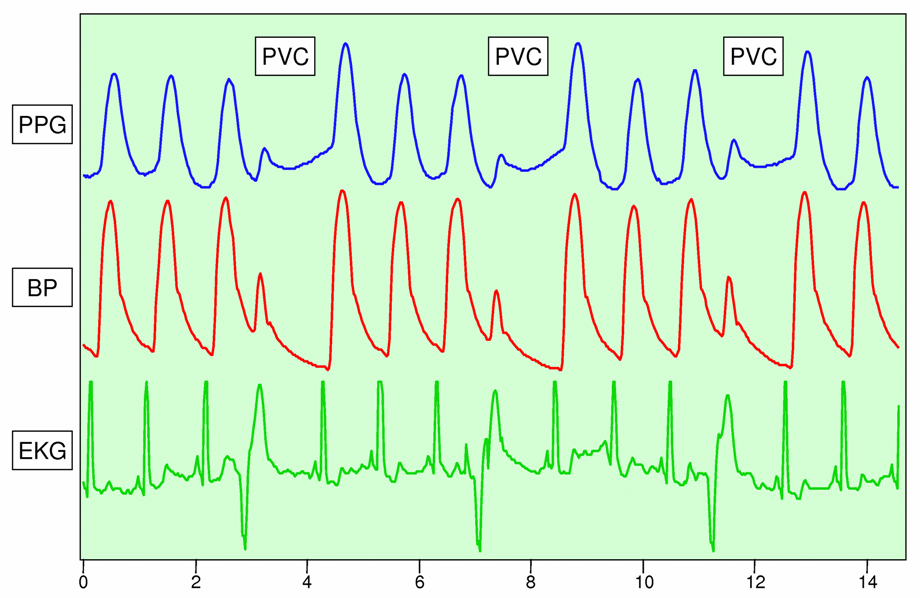
\includegraphics[width=0.7\textwidth, keepaspectratio=true]{chap6-PVC.png}
  \caption{Diagram of the layers of human skin.}
  \label{fig:chap6-PVC}
\end{figure}

%----------------------------------------------------------------------------------------
\section{The future study}

\begin{compactitem}
\item {Highly Dynamic Ambient Light Scenario}\cite {6799899}\\
Heart rate can be monitored remotely using regular RGB cameras by analyzing minute skin color changes caused
by periodic blood flow. I will study an infrared-based alternative for light-robust camera-based heart
rate measurements. It is possible to remotely measure heart rate using regular RGB cameras.
Heart rate is captured using remote photoplethysmography (remote PPG), which is an extension of the contact
photoplethysmography developed in the 1930s by Hertzman. The principle behind this
technology is that the light reflected from the skin is modulated according to the specific absorption
spectrum of the hemoglobin, the main constituent of blood. Each time the heart beats,
a new blood flow reaches the skin leading to minute variations of the skin color, so called micro-blushes.
While these micro-blushes cannot be observed by the human eye, regular camera and dedicated algorithms
allow their extraction. Results reported on remote PPG-based heart rate measurement have so far shown good
accuracy under stable light conditions for situations ranging from monitoring stationary subjects.
However, since remote PPG is based on the analysis of minute color changes, its performance in an
highly dynamic ambient light or dark setting using an RGB implementation is questionable.
The reason for concern is the highly dynamic and unpredictable environment especially in terms of lighting
conditions which can vary from (i) full to cloudy sunlight, (ii) natural to artificial light and (iii)
presence to absence of light. The amount and spectral content of the light available in the environment
are the main factors that need to be accounted for to achieve light robust camerabased heart rate measurements.
We will study an infrared-based implementation of remote PPG measurement suitable for the highly dynamic ambient light
environment and present results obtained under highly dynamic light
conditions.

\item {INFRARED-BASED REMOTE PPG}\\
As in full darkness RGB cameras do not function at all, we will study
an infrared-based remote PPG solution that uses a dedicated light source.
A light source emitting in the infrared region of the spectrum
(700nm to 1000nm) (i) ensures user comfort, as it is invisible to human
eye, and (ii) allows remote PPG measurements as the infrared region is
also modulated by the blood pulse.  Disturbances in the measurement caused
by external light sources are largely eliminated by using a narrowband
optical filter. The infrared light source is flashed in sync with the
camera frame rate. The flash duration and intensity are optimized such
that the total projected optical power complies with official safety
regulations. The extraction of the remote PPG waveform is performed by applying
spatio-temporal,  FFT, processing techniques.
To ensure that the processing takes into account only relevant pixels a
skin detection step is added. The extraction of the heart rate values from
the raw waveform is based on Fourier analysis.\cite{rPPG7005489}

\item{Future Study to combine both motion-robust and Ambient Light Immunity}

\begin{figure}[h]
  \centering
    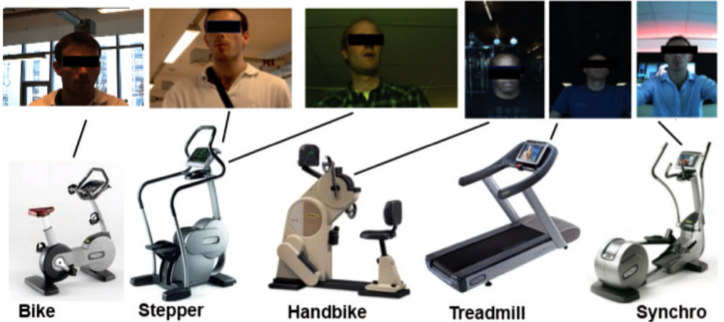
\includegraphics[width=0.7\textwidth, keepaspectratio=true]{chap6-rPPGMotion.png}
  \caption{Fitness devices and corresponding camera view to test motion robustness.}
  \label{fig:chap6-rPPGMotion}
\end{figure} \cite{rPPGPubMed}

\end{compactitem}
%----------------------------------------------------------------------------------------
%% Chapter 7
\chapter{Motion-Robust and Ambient Light Immune Remote PPG} % Main chapter title

\label{Chapter7} % For referencing the chapter elsewhere, use \ref{Chapter1}

\lhead{Chapter 7. \emph{Fundamental Mathematics}} % This is for the header on each page - perhaps a shortened title

%----------------------------------------------------------------------------------------
\section{Highly Dynamic Ambient Light Scenario}
Driving a car
Dark Room
Dancing Disco Party

\section{motion-robust rPPG}

\begin{compactitem}

\item Diagonal Matrix Properties
The time complexity is $O(N^2),  (C_2^N) = O(N^2/2)$.
\end{compactitem}

%----------------------------------------------------------------------------------------
\section{Future Study to combine both motion-robust and Ambient Light Immunity}

You have reached the end of this mini-guide. You can now rename or overwrite this pdf file and begin writing your own `\texttt{Chapter1.tex}' and the rest of your thesis. The easy work of setting up the structure and framework has been taken care of for you. It's now your job to fill it out!

Good luck and have lots of fun!


%----------------------------------------------------------------------------------------
%	THESIS CONTENT - APPENDICES
%----------------------------------------------------------------------------------------

\addtocontents{toc}{\vspace{2em}} % Add a gap in the Contents, for aesthetics

\appendix % Cue to tell LaTeX that the following 'chapters' are Appendices

% Include the appendices of the thesis as separate files from the Appendices folder
% Uncomment the lines as you write the Appendices

% Appendix A

\chapter{The Study List in PHD Program} % Main appendix title

\label{AppendixA} % For referencing this appendix elsewhere, use \ref{AppendixA}

\lhead{Appendix A. \emph{Appendix Title Here}} % This is for the header on each page - perhaps a shortened title

Write your Appendix content here.
%\input{Appendices/AppendixB}
%\input{Appendices/AppendixC}

\addtocontents{toc}{\vspace{2em}} % Add a gap in the Contents, for aesthetics

\backmatter

%----------------------------------------------------------------------------------------
%	BIBLIOGRAPHY
%----------------------------------------------------------------------------------------

\label{Bibliography}

\lhead{\emph{Bibliography}} % Change the page header to say "Bibliography"

\bibliographystyle{unsrtnat} % Use the "unsrtnat" BibTeX style for formatting the Bibliography

\bibliography{Bibliography} % The references (bibliography) information are stored in the file named "Bibliography.bib"

\end{document}